In diesem Kapitel wird die Umsetzung des Demonstrators dokumentiert.

Im Anhang~\ref{sec:photos} sind Fotos des Demonstrators abgelegt.

\pagebreak

\subsection{Firmware}

Der selbst entwickelte Firmware-Treiber für den \acrshort{tdc} befindet im Anhang~\ref{sec:tdc_driver}.

\pagebreak

\subsection{Schaltungen}
Nachfolgend werden sämtliche Teil-Schaltungen thematisiert, welche für das entwickelten \acrshort{tof}-Evaluationsmodul
nötig sind. Ein vollständiges Schema kann dem Anhang~\ref{sec:schematic_apdx} entnommen werden. Die kompletten
Projekt-Dateien sind im elektronischen Anhang dieses Projektes verfügbar.

Designt wurde das Schema mit Hilfe des Open-Source Tools \dq KiCad EDA 8.0\dq\ \cite{kicad2025kicadeda}.

\subsubsection{Selective Input Voltage}

Abbildung~\ref{fig:selective_input_voltage} zeigt die Beschaltung zur Selektion der Speisung.

\begin{figure}[H]
    \centering
    \includegraphics[page=2, trim=80 590 750 50, clip, width=0.9\textwidth]{attachments/schematic.pdf}
    \caption{Selective Input Voltage}\label{fig:selective_input_voltage}
\end{figure}

Für die Speisung des Nucleo-Boards bestehen die folgenden Möglichkeiten:

\begin{itemize}
    \item 5~V von USB-Buchse
    \item 5~V von externem Power-Supply (\lstinline|JP1| + \lstinline|JP2|)
    \item 12~V von externem Power-Supply (\lstinline|JP3|)
\end{itemize}

Siehe dazu auch Kapitel~\ref{sec:schematic_nucleo}.

Für die Speisung der 5~V Elektronik bestehen die folgenden Möglichkeiten:

\begin{itemize}
    \item 5~V von Nucleo-Board (\lstinline|JP1|)
    \item 5~V von externem Power-Supply (\lstinline|JP2|)
    \item 12~V von externem Power-Supply via Nucleo-Board (\lstinline|JP1| + \lstinline|JP3|)
\end{itemize}

Für die Speisung der Photodiode bestehen die folgenden Möglichkeiten:

\begin{itemize}
    \item 5~V von 5~V-Elektronik (\lstinline|SW2| Position 3)
    \item 12~V von externem Power-Supply (\lstinline|SW2| Position 1)
\end{itemize}

Siehe dazu auch Kapitel~\ref{sec:schematic_photo_receiver}.

\subsubsection{Nucleo Board}\label{sec:schematic_nucleo}

Die Beschaltung des NUCLEO-F042K6 Boards \cite{st2024nucleof042k6_usermanual} ist in Abbildung~\ref{fig:nucleo_board}
gezeigt.

\begin{figure}[H]
    \centering
    \includegraphics[page=2, trim=530 580 300 50, clip, width=0.9\textwidth]{attachments/schematic.pdf}
    \caption{Nucleo Board}\label{fig:nucleo_board}
\end{figure}

Das NUCLEO Board ist ein sogenanntes \dq Development-Kit\dq, welches eine STM32F042K6 \acrshort{mcu}
beinhaltet. Am Rand des Boards werden diverse Pins der \acrfull{mcu} via Pin-Header
einfach zur Verfügung gestellt. Dies erleichtert die Integration in eine eigene Elektronik
enorm. Programmiert wird die \acrshort{mcu} über eine \acrshort{usb}-Schnittstelle.

In diesem Design wird das Entwicklerboard dazu benötigt, die TDC7200 ICs zu
bedienen. Dazu wird einerseits ein \acrfull{spi} benötigt, um die Mess-ICs zu konfigurieren
und auch auszulesen (siehe SPI-Bus in der Abbildung). Weiter können auf beiden \acrshort{tdc}s Messungen
gestartet werden mit den Signalen \lstinline|start_ele|, resp. \lstinline|start_opt|. Für den
\acrshort{tdc} welcher sich um die elektrischen Signale kümmert kann zudem mit \lstinline|stop_ele| ein
Stopp-Puls generiert werden.
Zu guter Letzt ist das NUCLEO dafür zuständig, die Laser-Diode anzusteuern, was mit den Signalen
\lstinline|LD_pulse| sowie $\overline{\mbox{\lstinline|LD_enable|}}$ geschieht.

\subsubsection{TDC Electrical Signal}

Die Beschaltung des TDC7200 \cite{ti2016tdc7200_datasheet} für den elektrischen Teil ist in
Abbildung~\ref{fig:tdc_ele_signal} gezeigt.

\begin{figure}[H]
    \centering
    \includegraphics[page=2, trim=80 330 750 310, clip, width=0.9\textwidth]{attachments/schematic.pdf}
    \caption{\acrshort{tdc} Electrical Signal}\label{fig:tdc_ele_signal}
\end{figure}

Der TDC7200 ist über die die Start- und Stopp-Leitungen, ein Enable-Signal sowie die \acrshort{spi}-Leitungen mit der
\acrshort{mcu} verbunden.

Wie bereits im Kapitel~\ref{sec:approach} angesprochen, wird der elektrische \acrshort{tdc} dazu verwendet, den Chip
erstmalig in Betrieb zu nehmen und sich damit vertraut zu machen. Am Anschluss \lstinline|J3| kann in einem nächsten
Schritt ein beliebig langes Kabel angeschlossen werden. Dies ermöglicht es, erste Messresultate, natürlich rein elektrisch,
vom TDC7200 auszulesen.

Mittels Schalter \lstinline|SW1| kann das \lstinline|STOP|-Signal wahlweise via \lstinline|stop_ele| oder
\lstinline|start_ele| generiert werden. Dies bietet zum einen die Möglichkeit, die Zeit zwischen dem Schalten von zwei
\acrshort{gpio}s zu messen. Zum anderen, kann derselbe \acrshort{gpio}-Pin zum Generieren des \lstinline|START|- und
\lstinline|STOP|-Signals verwendet werden, wodurch von der Verzögerungszeit direkt auf die Kabellänge an \lstinline|J3|
geschlossen werden kann.

\subsubsection{TDC Optical Signal}

Die Beschaltung des TDC7200 \cite{ti2016tdc7200_datasheet} für den optischen Teil ist in
Abbildung~\ref{fig:tdc_opt_signal} gezeigt.

\begin{figure}[H]
    \centering
    \includegraphics[page=2, trim=530 330 300 310, clip, width=0.9\textwidth]{attachments/schematic.pdf}
    \caption{\acrshort{tdc} Optical Signal}\label{fig:tdc_opt_signal}
\end{figure}

Die Beschaltung des \acrshort{tdc}s für die optische Messung gestaltet sich praktisch gleich wie beim elektrischen
Gegenstück. Der Hauptunterschied ist, hier aber, dass dessen \lstinline|STOP|-Signal nicht von der \acrshort{mcu} selber generiert
wird, sondern von einem Komparator, welcher am Ende des optischen Messpfades steht. Da der Komparator mit einem 5~V Pegel
arbeitet, ist der Spannungsteiler \lstinline|R1| / \lstinline|R2| vonnöten, welcher den 5~V Puls auf die geeigneten 3.3~V
herunterteilt.

\subsubsection{Oscillator For TDCs}

Die Beschaltung des Oszillators für die beiden \acrshort{tdc} ist in Abbildung~\ref{fig:oscillator_tdc} gezeigt. Es
handelt sich hierbei um einen normalen Quartz-Oszillator mit integriertem Schwingkreis. Praktischerweise ist bei diesem
also keine weitere Beschaltung notwendig.

\begin{figure}[H]
    \centering
    \includegraphics[page=2, trim=80 90 930 550, clip, width=0.45\textwidth]{attachments/schematic.pdf}
    \caption{Oscillator for \acrshort{tdc}s}\label{fig:oscillator_tdc}
\end{figure}

\subsubsection{Power Supply Separation}

Für die Beschaltung der Photodiode, inkl. \acrshort{tia} und Komparator, macht es Sinn eine Spannungsversorgung mit
möglichst wenig Rauschen zu haben.

Dazu wurde die Separierung vorgenommen, welche in Abbildung~\ref{fig:power_supply_separation} dargestellt ist.

\begin{figure}[H]
    \centering
    \includegraphics[page=2, trim=260 90 640 550, clip, width=0.7\textwidth]{attachments/schematic.pdf}
    \caption{Power Supply Separation}\label{fig:power_supply_separation}
\end{figure}

Prinzipiell sollen die Speisungen über eine Ferrit-Perle etwas entstört werden. Massgeblich ist hier natürlich auch der
physikalische Verlauf des Speisungspfades auf dem Layout. Dazu mehr im entsprechenden Kapitel~\ref{sec:layout}. Wahlweise
besteht nebst den Ferrit-Perlen die Möglichkeit, mittels Kondensatoren die Speisung weiter zu entkoppeln. Es wird jedoch
davon ausgegangen, dass dies in einem ersten Schritt nicht notwendig ist.

\subsubsection{Laser Driver}\label{sec:schematic_laser_driver}

Die Laser Diode RLD65NZX1 \cite{rohm2019rld65nzx1_datasheet} wird mittels Lasertreiber LMG1025-Q1 \cite{ti2024lmg1025q1_datasheet}
und NexFET \cite{ti2016csd17578q3a_datasheet} angesteuert. Für die Generierung eines kurzen Pulses (0.5 \dots 100~ns)
wurde mittels Hochpass und AND-Gatter \cite{diodes202074lvc1g08q_datasheet} implementiert. Siehe dazu Abbildung~\ref{fig:laser_driver}.

Der Widerstand \lstinline|R25| bildet den Vorwiderstand für die Laser-Diode, welcher sich gemäss der Formel~\ref{eq:ld_resistor} berechnet.

\begin{equation}\label{eq:ld_resistor}
    R_{v} = \frac{V_{cc} - V_{fld}}{I_{ld}} = \frac{5~V - 2~V}{40~mA} = 75~\Omega
\end{equation}

Im Schema eingezeichnet ist aktuell ein Platzhalterwert. Während der Inbetriebnahme wird der Widerstand je nach Bedarf
verändert. Wird dieser beispielsweise verkleinert, so vergrössert sich der Strom durch die Laser-Diode und somit die ausgesandte
Lichtleistung.

%TODO Erwähnen was für ein Widerstand schlussendlich verwendet wurde. z.B. 10x Überansteuerung weil kleiner Duty-Cycle.

\begin{figure}[H]
    \centering
    \includegraphics[page=3, trim=100 520 550 60, clip, width=0.9\textwidth]{attachments/schematic.pdf}
    \caption{Laser Driver}\label{fig:laser_driver}
\end{figure}

\subsubsection{Photo Receiver}\label{sec:schematic_photo_receiver}

Um den Photostrom der Photodiode NJL6401R \cite{jrc2014njl6401r3_datasheet} zu verstärken und in eine Spannung umzuwandeln,
wurde mit dem Operationsverstärker OPA858 \cite{ti2018opa858_datasheet} ein Transimpedanzverstärker aufgebaut. Der
Ausgang des Transimpedanzverstärkers geht auf den Komparator TLV3501 \cite{ti2016tlv3501_datasheet}, um das \lstinline|STOP|-Signal
für den \acrshort{tdc} zu generieren. Siehe dazu Abbildung~\ref{fig:photo_receiver}.

Der Feedback-Widerstand \lstinline|R26| kann je nach bedarf verändert werden. Wird dieser vergrössert, so steigt auch der
negative Puls am Ausgang des \acrshort{tia}s. Mit \lstinline|C20| kann zudem bei Bedarf eine kleine Kapazität hinzugefügt
werden. Diese hat zum Ziel, ein Schwingen des Verstärkers zu unterdrücken, falls dieser eine Neigung zum Schwingen haben
sollte.

\begin{figure}[H]
    \centering
    \includegraphics[page=3, trim=100 240 600 340, clip, width=0.9\textwidth]{attachments/schematic.pdf}
    \caption{Photo Receiver}\label{fig:photo_receiver}
\end{figure}

\subsubsection{Decoupling Capacitors}

Die Beschaltung der Entkopplungs-Kondensatoren ist in Abbildung~\ref{fig:decoupling_capacitors} dargestellt. Die
Kondensatoren für den Operationsverstärker OPA858 und für den Komparator TLV3501 wurden dem Vorschlag im Datenblatt
entnommen. Zusätzlich wird auch der Gate-Treiber beim Laser-Treiber mit einer zusätzlichen, grösseren Kapazität gestützt,
was sich positiv auf die Stabilität der Speisung auswirken sollte.

\begin{figure}[H]
    \centering
    \includegraphics[page=3, trim=100 60 650 630, clip, width=0.9\textwidth]{attachments/schematic.pdf}
    \caption{Decoupling Capacitors}\label{fig:decoupling_capacitors}
\end{figure}

\pagebreak

\subsection{Layout}\label{sec:layout}

In diesem Kapitel werden die \acrshort{pcb}-Layouts dokumentiert.

\subsubsection{Kupfer-Layer}

\begin{figure}[H]
    \centering
    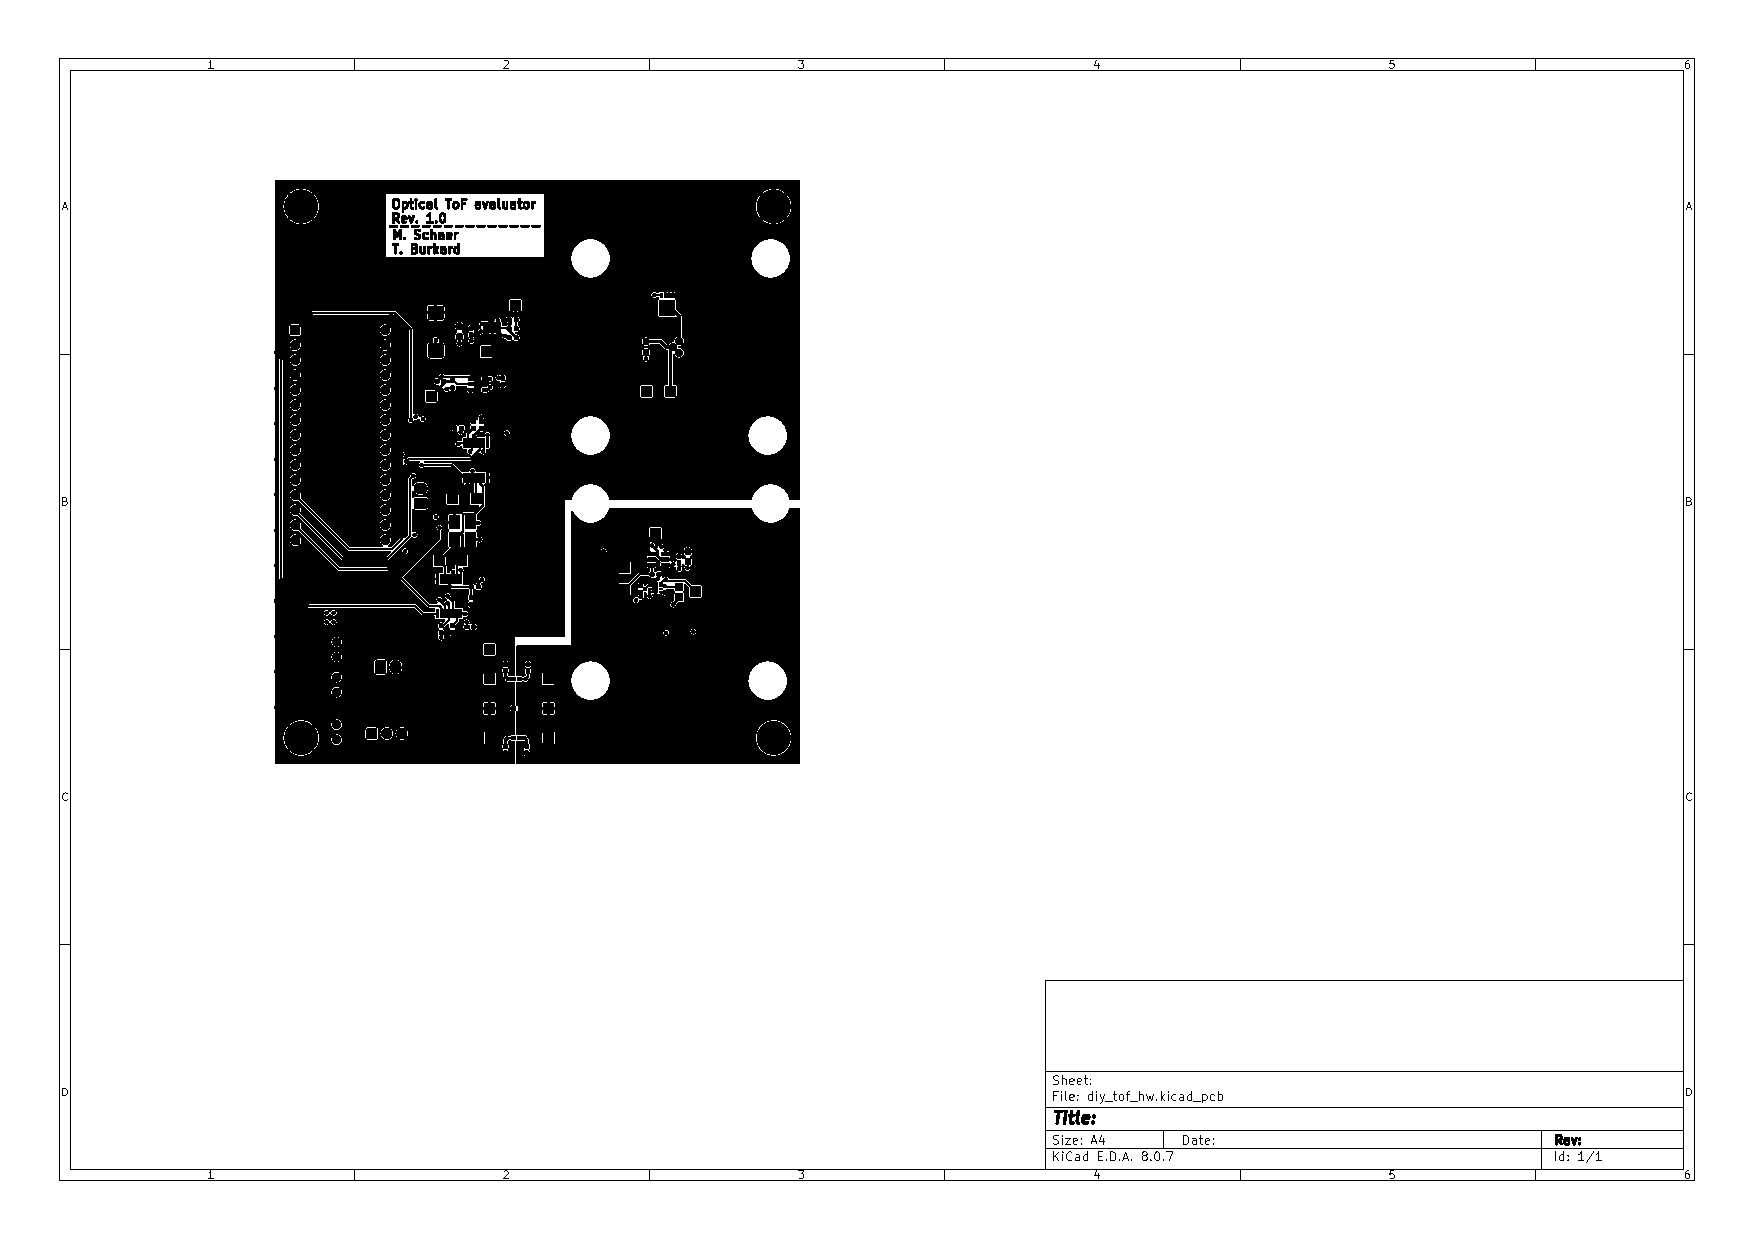
\includegraphics[trim=130 220 450 80, clip, width=0.6\textwidth]{attachments/pcb_F_Cu.pdf}
    \caption{PCB Layout Top}\label{fig:pcb_f_cu}
\end{figure}

\begin{figure}[H]
    \centering
    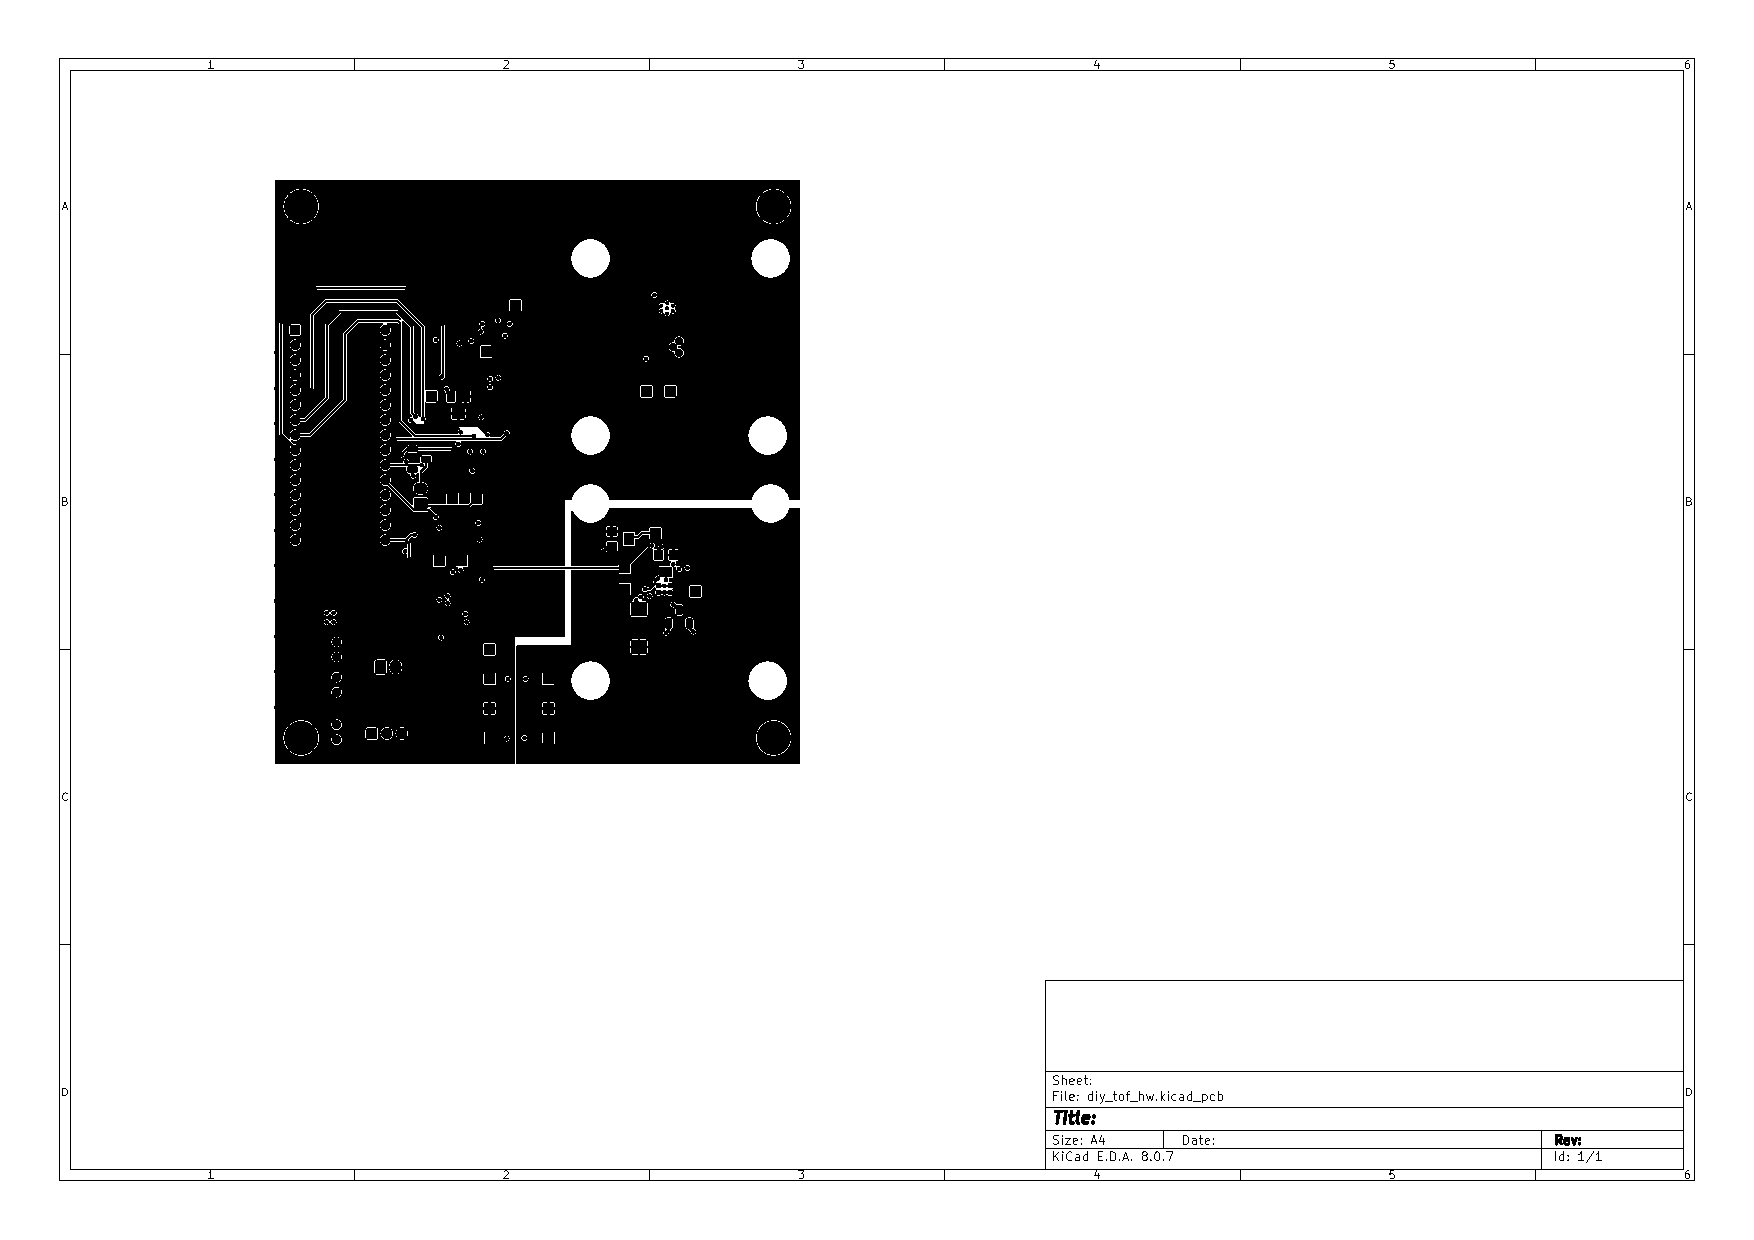
\includegraphics[trim=130 220 450 80, clip, width=0.6\textwidth]{attachments/pcb_B_Cu.pdf}
    \caption{PCB Layout Bottom}\label{fig:pcb_b_cu}
\end{figure}

\begin{figure}[H]
    \centering
    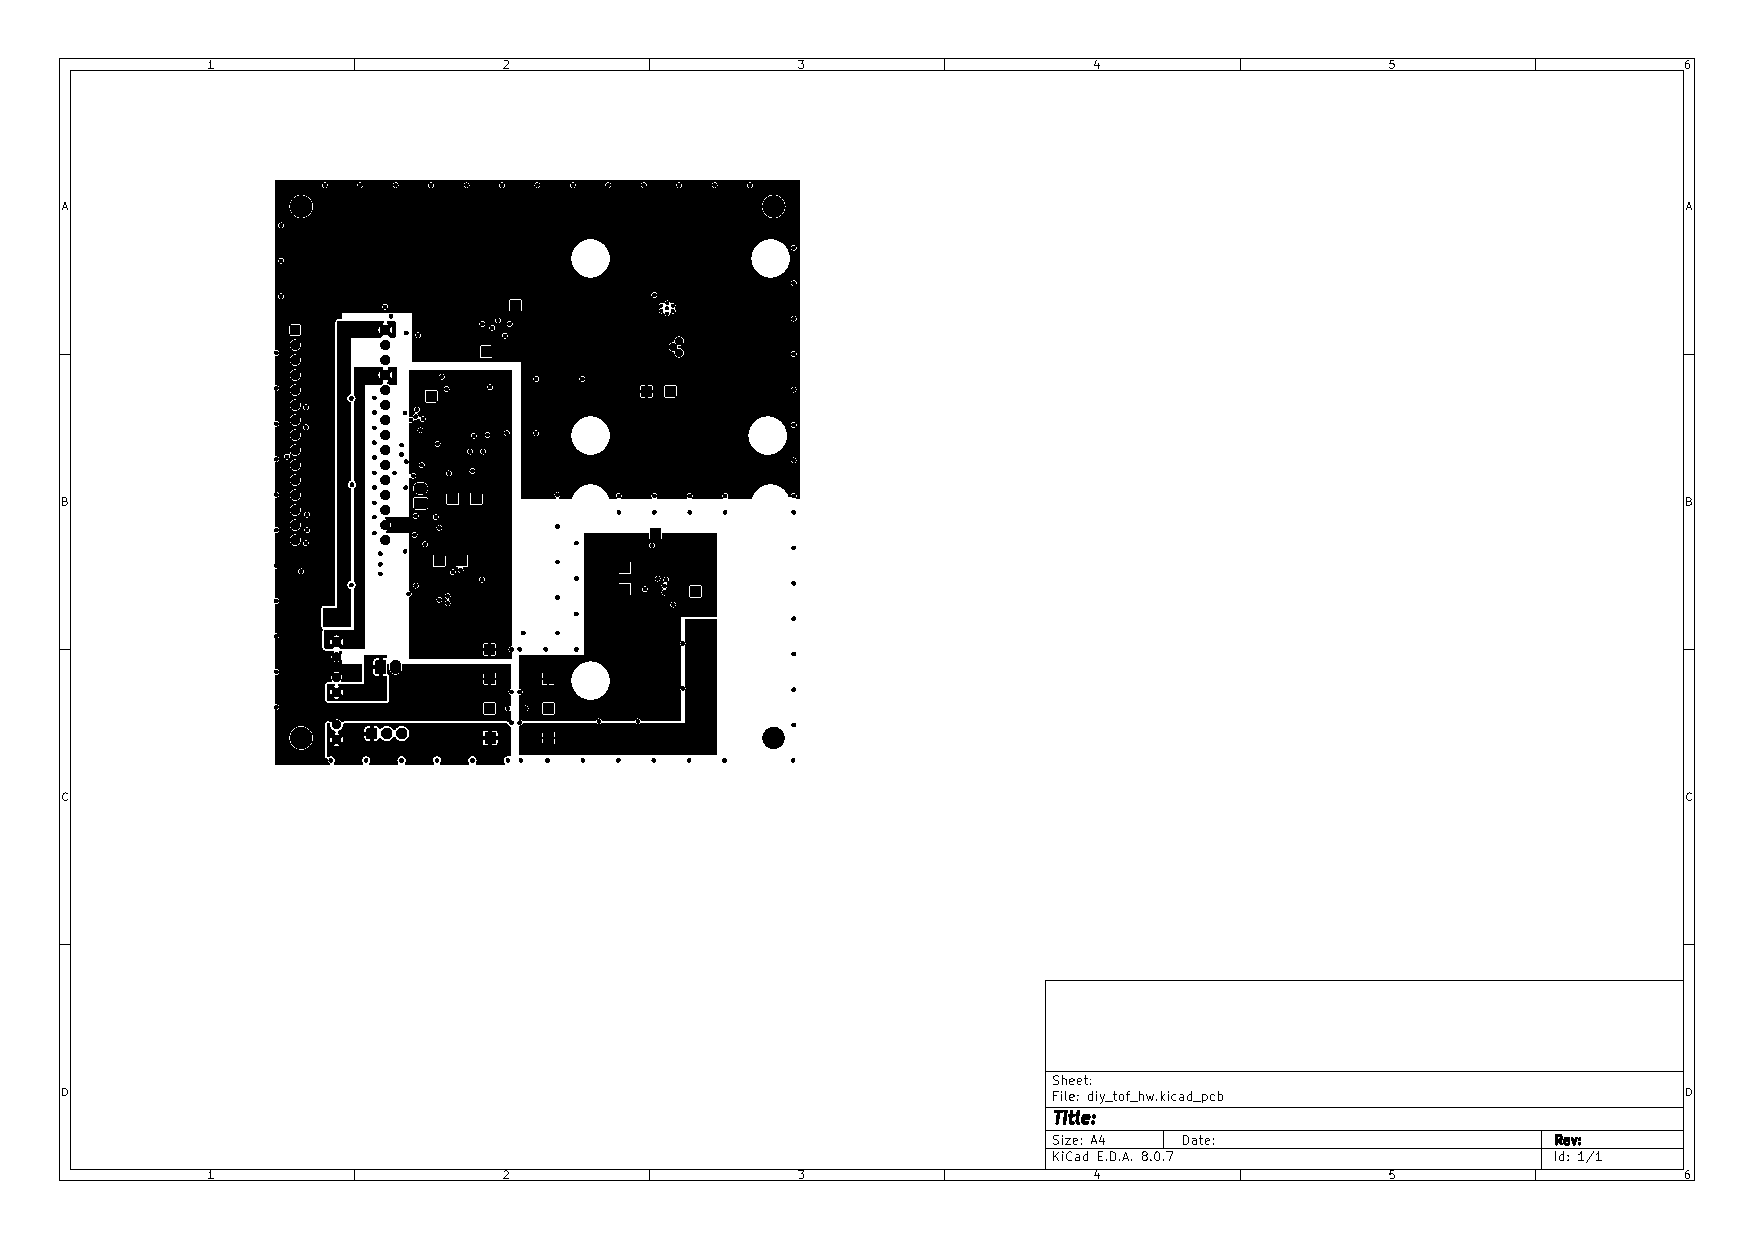
\includegraphics[trim=130 220 450 80, clip, width=0.6\textwidth]{attachments/pcb_In1_Cu.pdf}
    \caption{PCB Layout Innen 1}\label{fig:pcb_in1_cu}
\end{figure}

\begin{figure}[H]
    \centering
    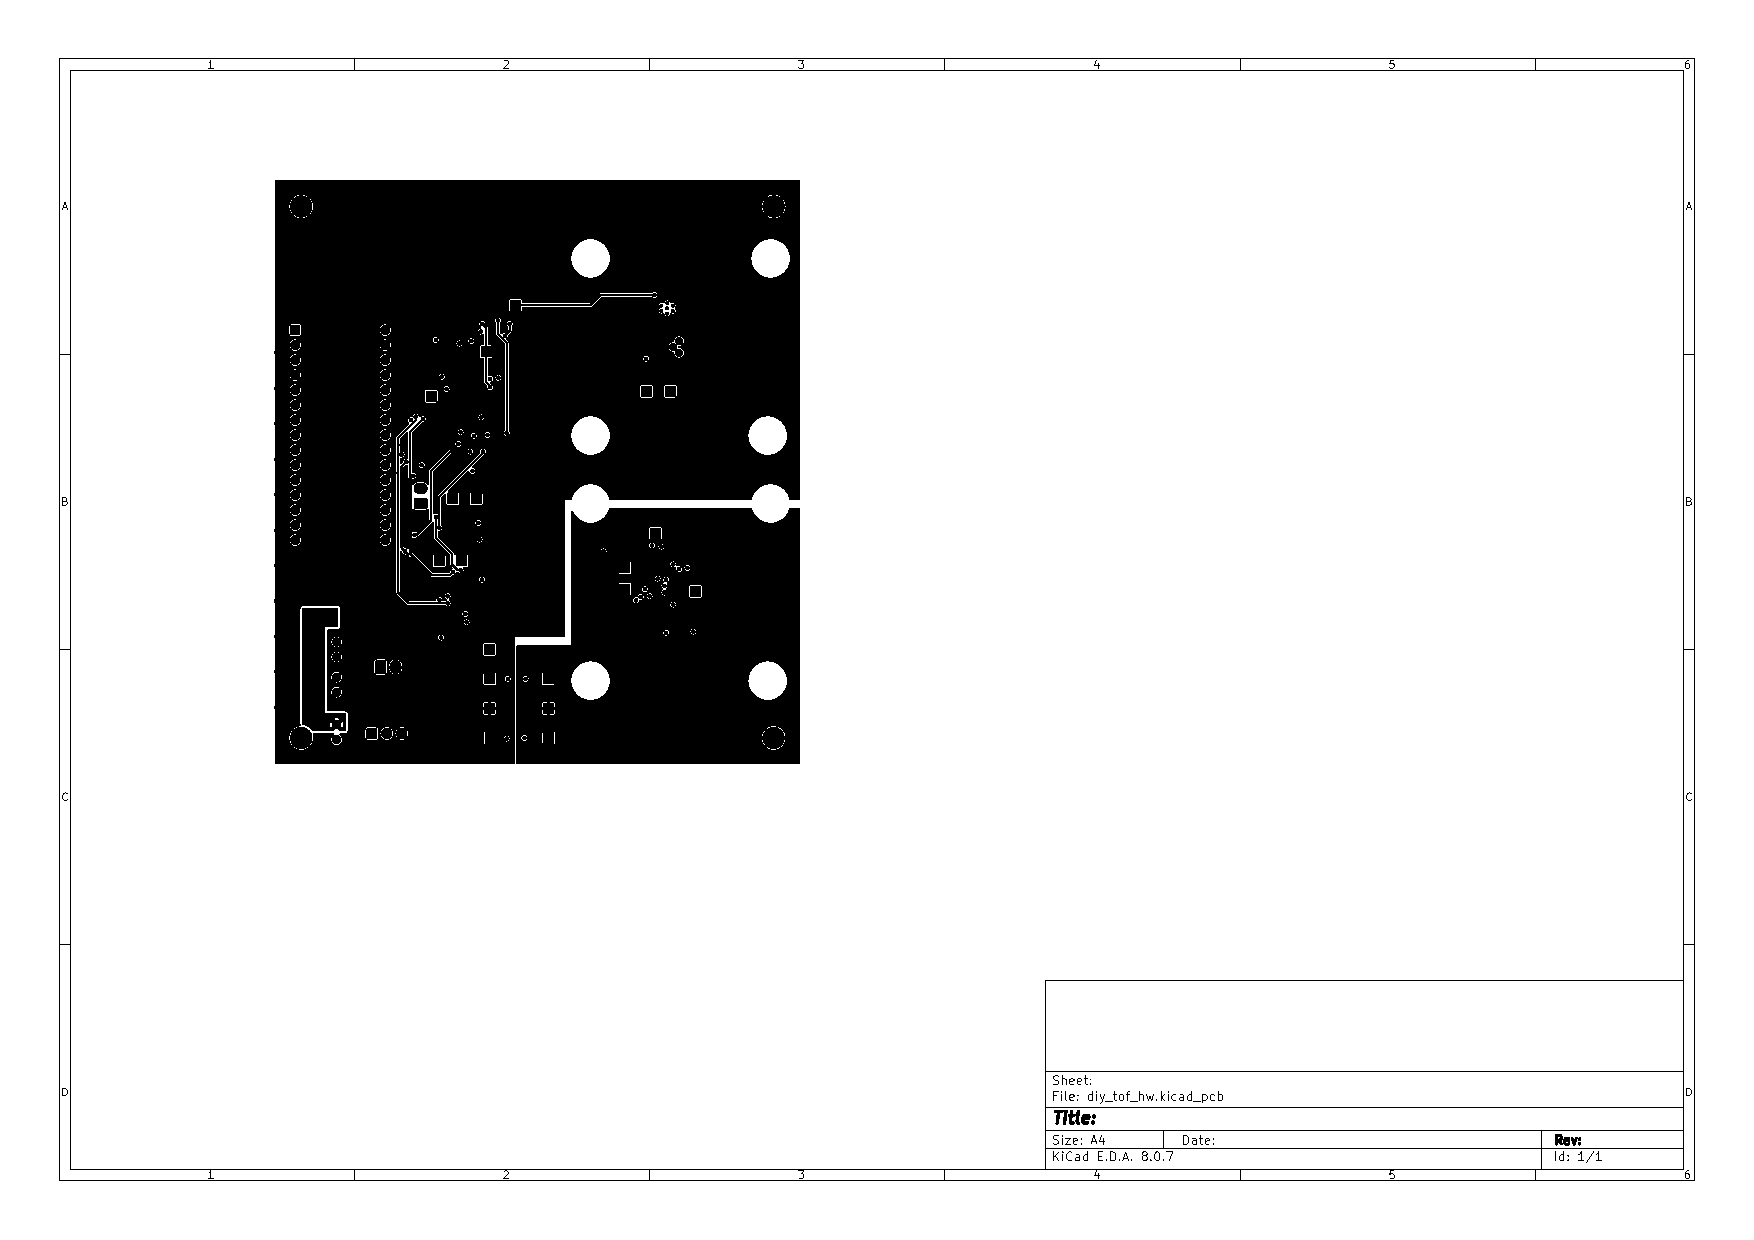
\includegraphics[trim=130 220 450 80, clip, width=0.6\textwidth]{attachments/pcb_In2_Cu.pdf}
    \caption{PCB Layout Innen 2}\label{fig:pcb_in2_cu}
\end{figure}

\subsubsection{Komponenten-Platzierung}

\begin{figure}[H]
    \centering
    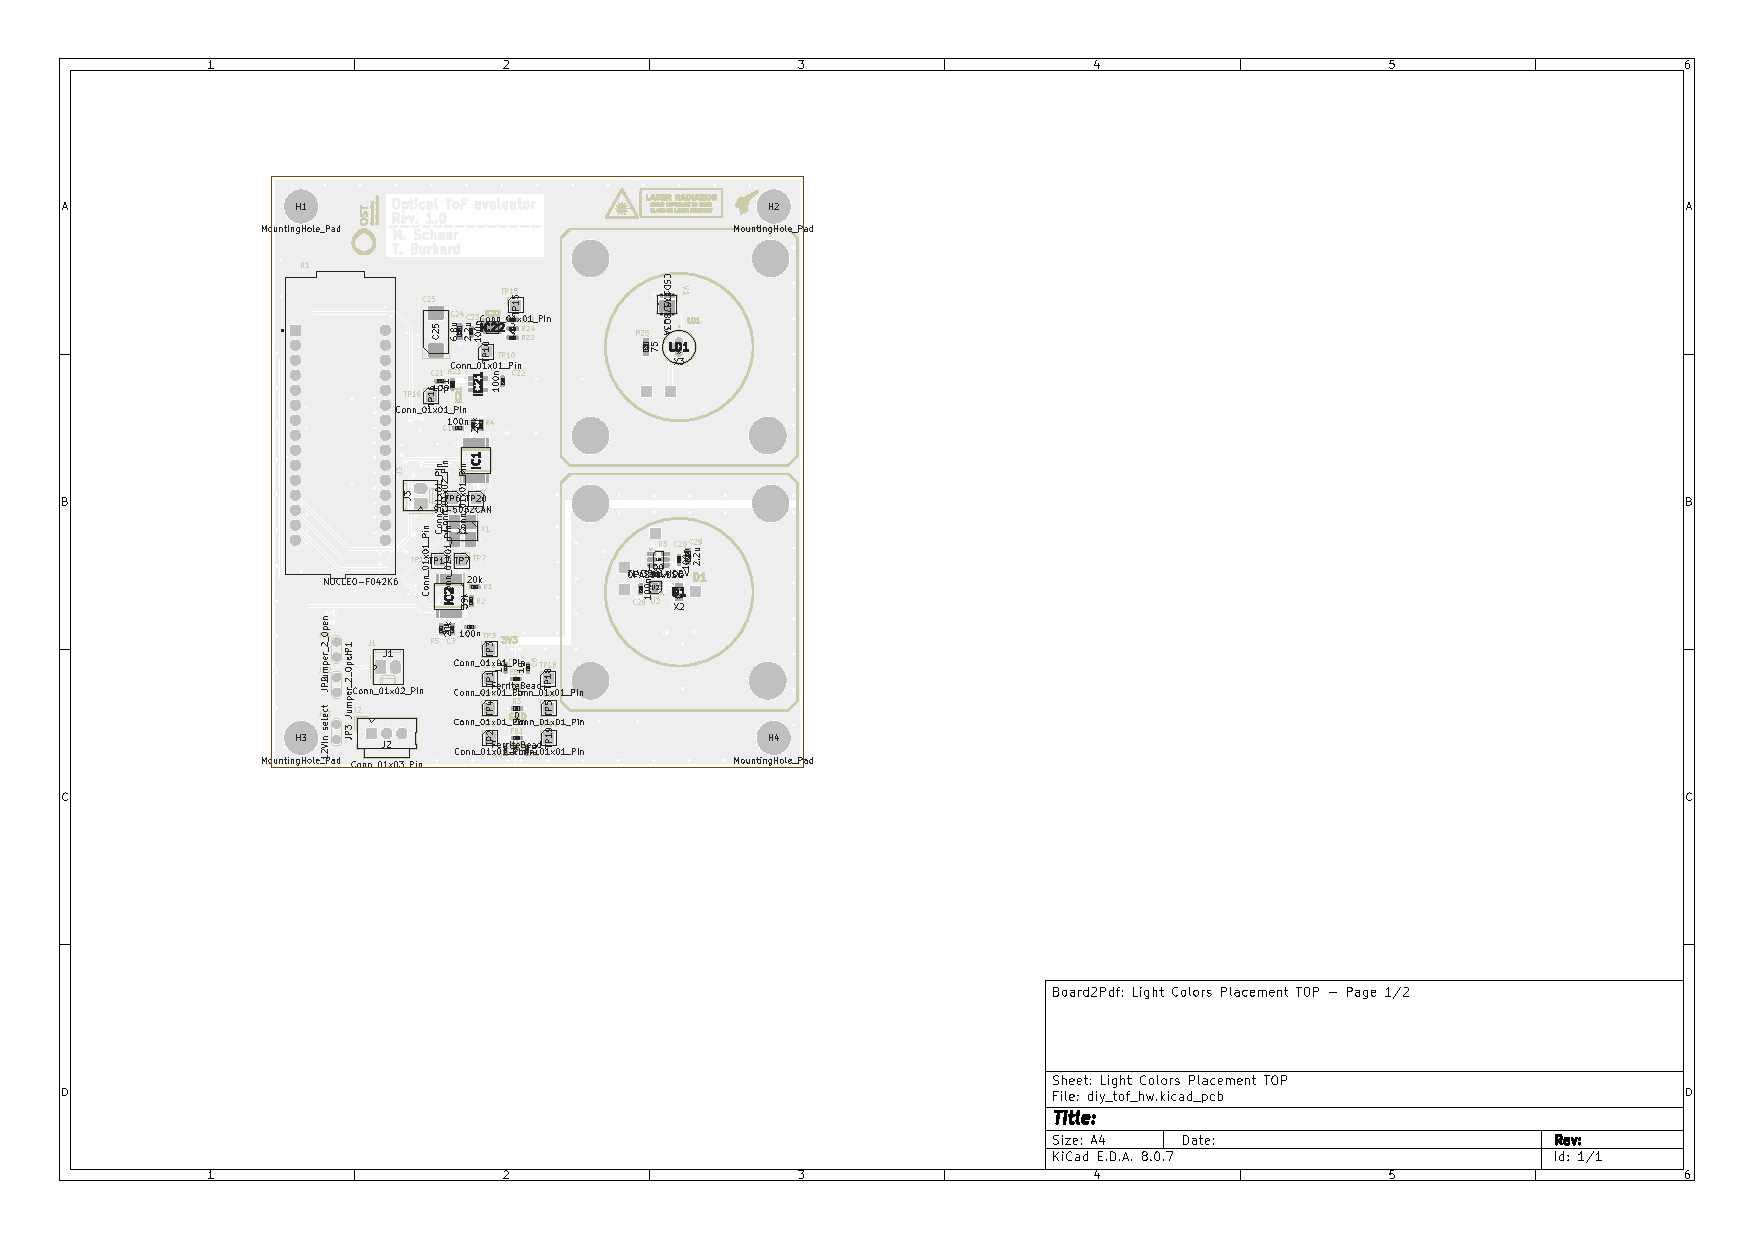
\includegraphics[page=1, trim=120 220 450 80, clip, width=0.6\textwidth]{attachments/pcb_placement.pdf}
    \caption{PCB Komponenten-Platzierung Top}\label{fig:pcb_placement_1}
\end{figure}

\begin{figure}[H]
    \centering
    \includegraphics[page=2, trim=450 220 120 80, clip, width=0.6\textwidth]{attachments/pcb_placement.pdf}
    \caption{PCB Komponenten-Platzierung Bottom}\label{fig:pcb_placement_2}
\end{figure}

\pagebreak

\subsection{3D View}

\begin{figure}[H]
    \centering
    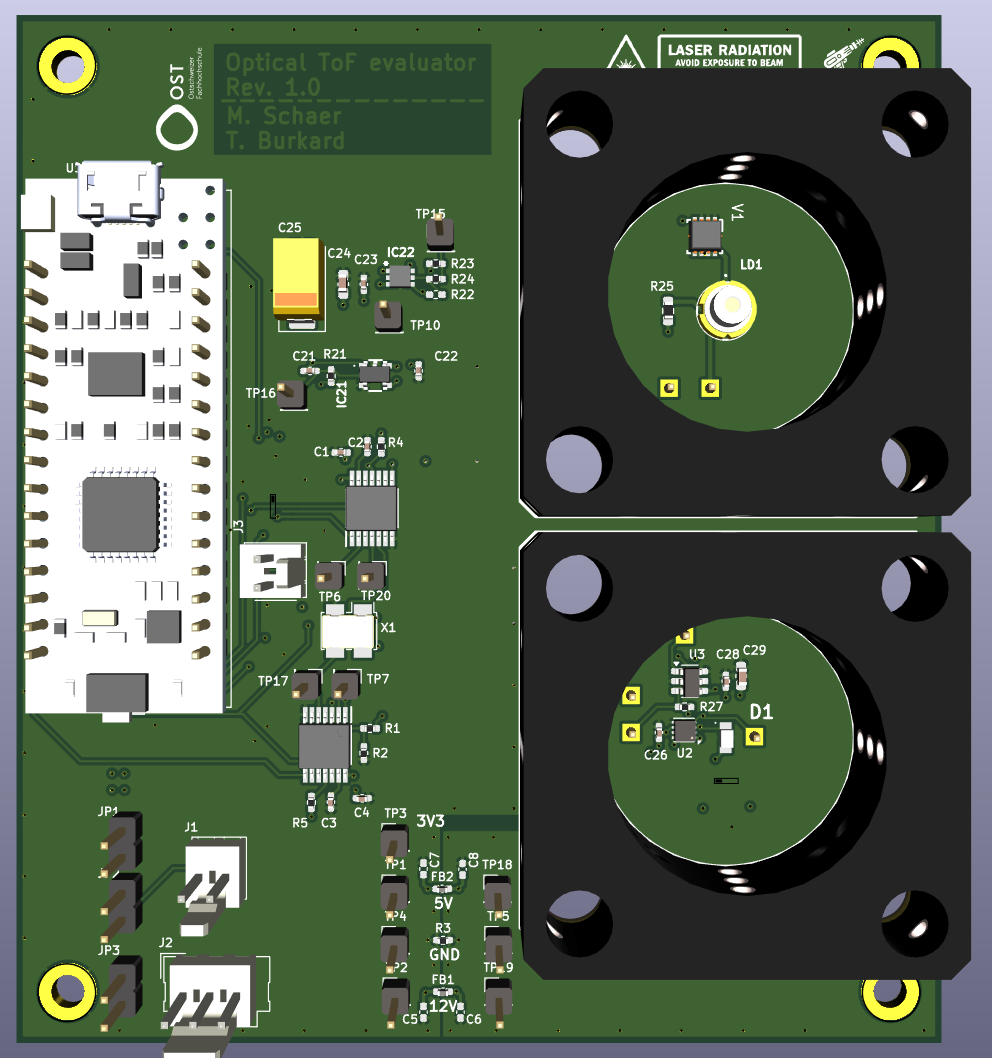
\includegraphics[width=0.6\textwidth]{graphics/3d_top.png}
    \caption{3D View Top}\label{fig:3d_top}
\end{figure}

\begin{figure}[H]
    \centering
    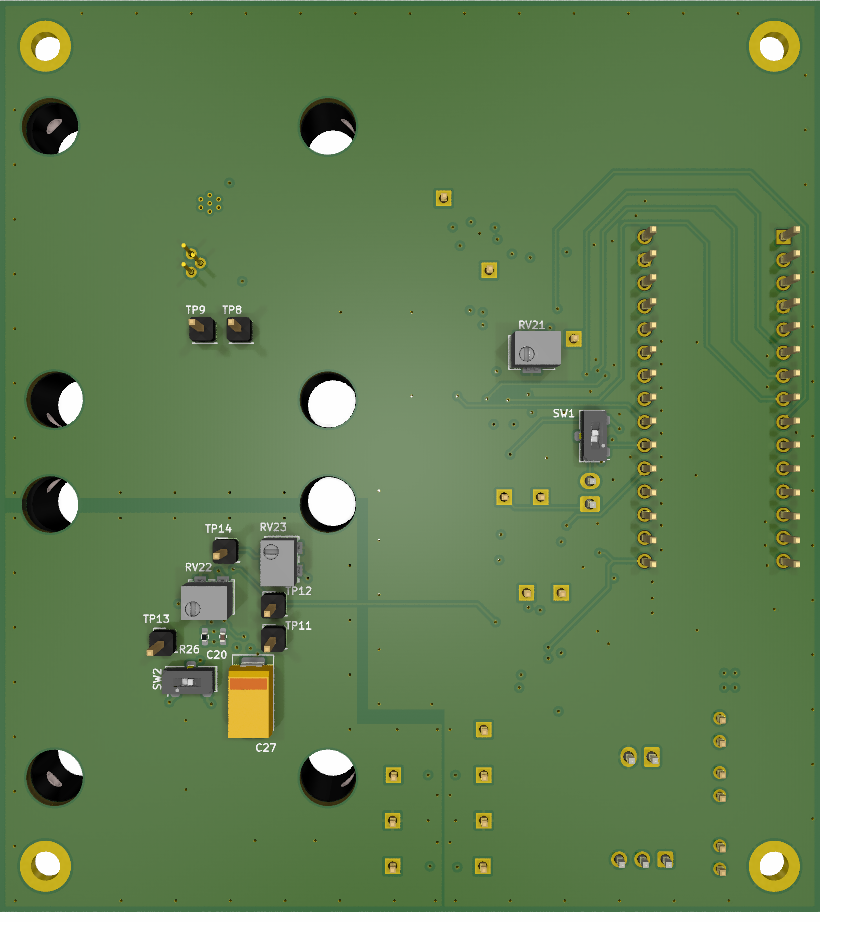
\includegraphics[width=0.6\textwidth]{graphics/3d_bottom.png}
    \caption{3D View Bottom}\label{fig:3d_bottom}
\end{figure}
